\documentclass[xcolor=svgnames,compress]{beamer}

% see http://tex.stackexchange.com/questions/13423/how-to-color-href-links-in-beamer
\hypersetup{colorlinks,linkcolor=,urlcolor=alert}

\mode<presentation>
{
  \usetheme{Warsaw}
  \setbeamertemplate{navigation symbols}{}
  \setbeamercovered{dynamic}
}

\usepackage[spanish,es-noshorthands]{babel}
\usepackage[utf8x]{inputenc}
\usepackage[T1]{fontenc}
\usepackage{csquotes}
\usepackage{tikz}
\usepackage{fancyvrb}
\usepackage[htt]{hyphenat}

\PrerenderUnicode{áéíóúÁÉÍÓÚçÇ}

\title[Pósters científicos]{¿Cómo elaborar un buen póster científico?}
\author{Antonio García Domínguez}
\date{Cursos de doctorado \\ \small 18 de enero de 2012}
\institute{Universidad de Cádiz \\\vspace{2em} 
\includegraphics{cc-by-sa}}

\AtBeginSection[]
{
  \begin{frame}<beamer>{Contenidos}
    \tableofcontents[currentsection,hideothersubsections]
  \end{frame}
}

\AtBeginSubsection[]
{
  \begin{frame}<beamer>{Contenidos}
    \tableofcontents[currentsection,subsectionstyle=show/shaded/hide]
  \end{frame}
}

\usetikzlibrary{calc,positioning,shapes,shapes.geometric}

\begin{document}

\begin{frame}
  \titlepage
\end{frame}

\begin{frame}{Contenidos}
  \tableofcontents[hideallsubsections]

  Materiales:
  \begin{itemize}
  \item \url{http://github.com/bluezio/phd-posters-session}
  \item Campus Virtual de la UCA
  \end{itemize}
\end{frame}

\section[Conceptos]{¿En qué consiste?}
\label{sec:en-que-consiste}

\begin{frame}{¿Qué es una sesion de pósters científicos?}

  \begin{block}{Pasos usuales}
    \begin{enumerate}
    \item Cada autor elabora un póster que transmite de un vistazo lo
      que está investigando y sus resultados hasta la fecha
    \item El póster se coloca en un espacio especialmente habilitado
      (cerca de la comida o en un lugar de paso obligado)
    \item En las sesiones de pósters, los autores deben situarse al
      lado del póster para atender a las consultas de los asistentes
    \item Al terminar el evento, nos podemos traer el póster y
      reutilizarlo para presentar nuestra investigación a visitantes
    \end{enumerate}
  \end{block}

  \begin{block}{¿Por qué molestarse en hacerlo bien?}
    Un póster interesante, bien elaborado y bien defendido atraerá
    muchas más consultas y futuras colaboraciones.
  \end{block}

\end{frame}

\begin{frame}{¿Cómo se compara un póster con una ponencia normal?}

  \begin{block}{Situaciones habituales}
    \begin{itemize}
    \item Algunos eventos piden pósters para trabajos preliminares y
      artículos regulares para trabajos más avanzados
    \item Otros eventos lo consideran otra forma más de presentar el
      trabajo, en vez de una ponencia, y dejan escoger
    \end{itemize}
  \end{block}

  \begin{block}{¿Cuándo conviene más un póster?}
    \begin{itemize}
    \item Una ponencia regular es cómoda para explicar los resultados,
      pero es difícil seguirla y dar buena realimentación dentro de
      los 5' habituales de preguntas
    \item Los asistencias pueden leer un póster a su ritmo, y si
      tienen alguna duda pueden preguntar de forma más relajada
    \item Un póster da mayor libertad a la hora de expresarse
    \end{itemize}
  \end{block}
  
\end{frame}

\begin{frame}{Desventajas de un póster}

  \begin{block}{Impacto en el currículum}
    \begin{itemize}
    \item Una publicación de póster se considera menos valiosa que una
      publicación regular en algunas organizaciones
    \item Para que sea rentable el trabajo, eventualmente tendrá que
      ir a una revista científica
    \end{itemize}
  \end{block}

  \begin{block}{Eventos con mala organización}
    \begin{itemize}
    \item Algunos eventos le dan poco tiempo a las sesiones de
      pósters, dejándolo para las últimas horas del día y/o los
      \emph{coffee break}
    \item Otros eventos no motivan a los autores/asistentes a ir a las
      sesiones, y hay pósters sin nadie que los defienda o nadie que
      los discuta
    \end{itemize}
  \end{block}

\end{frame}

\section{Contenido}

\begin{frame}{Información habitual en un póster}

  \begin{block}{Indicad quiénes sois, de dónde venís y cómo contactaros}
    \begin{itemize}
    \item Nombre y apellidos (cuidado con las convenciones inglesas)
    \item Departamento, universidad y grupo de investigación (+ logos)
    \item Teléfono y e-mail de contacto
    \item Perfiles públicos en la Web (Twitter, sitio web personal, etc.)
    \end{itemize}
  \end{block}

  \begin{block}{Resumid el trabajo (para leer en 10' máximo)}
    \begin{itemize}
    \item ¿Cuál es el problema?
    \item ¿Por qué merece la pena resolverlo?
    \item ¿Qué es lo que proponéis?
    \item ¿Es buena vuestra idea?
    \item ¿Dónde encaja entre los demás trabajos dedicados a esto?
    \item ¿Qué tenéis pensado hacer a partir de ahora?
    \end{itemize}
  \end{block}

\end{frame}

\begin{frame}{¿A quién va dirigido el póster?}
  
\end{frame}

\begin{frame}{¿Cómo se evita abrumar a la audiencia?}
  \url{http://www.flickr.com/photos/somayalangley/2565759527/}
\end{frame}

\section{Formato}

\subsection{Diseño visual}

\begin{frame}{Distribución de los elementos}
  
\end{frame}

\begin{frame}{Esquemas de colores}
  
\end{frame}

\begin{frame}{Fuentes y formatos de imágenes}
  
\end{frame}

\begin{frame}{Gráficas utilizadas}
  
\end{frame}

\begin{frame}{Software a emplear}
  
\end{frame}

\subsection{Impresión y montaje}

\begin{frame}{Tamaños habituales}
  \begin{columns}
    \column{.5\textwidth}

    \begin{center}
      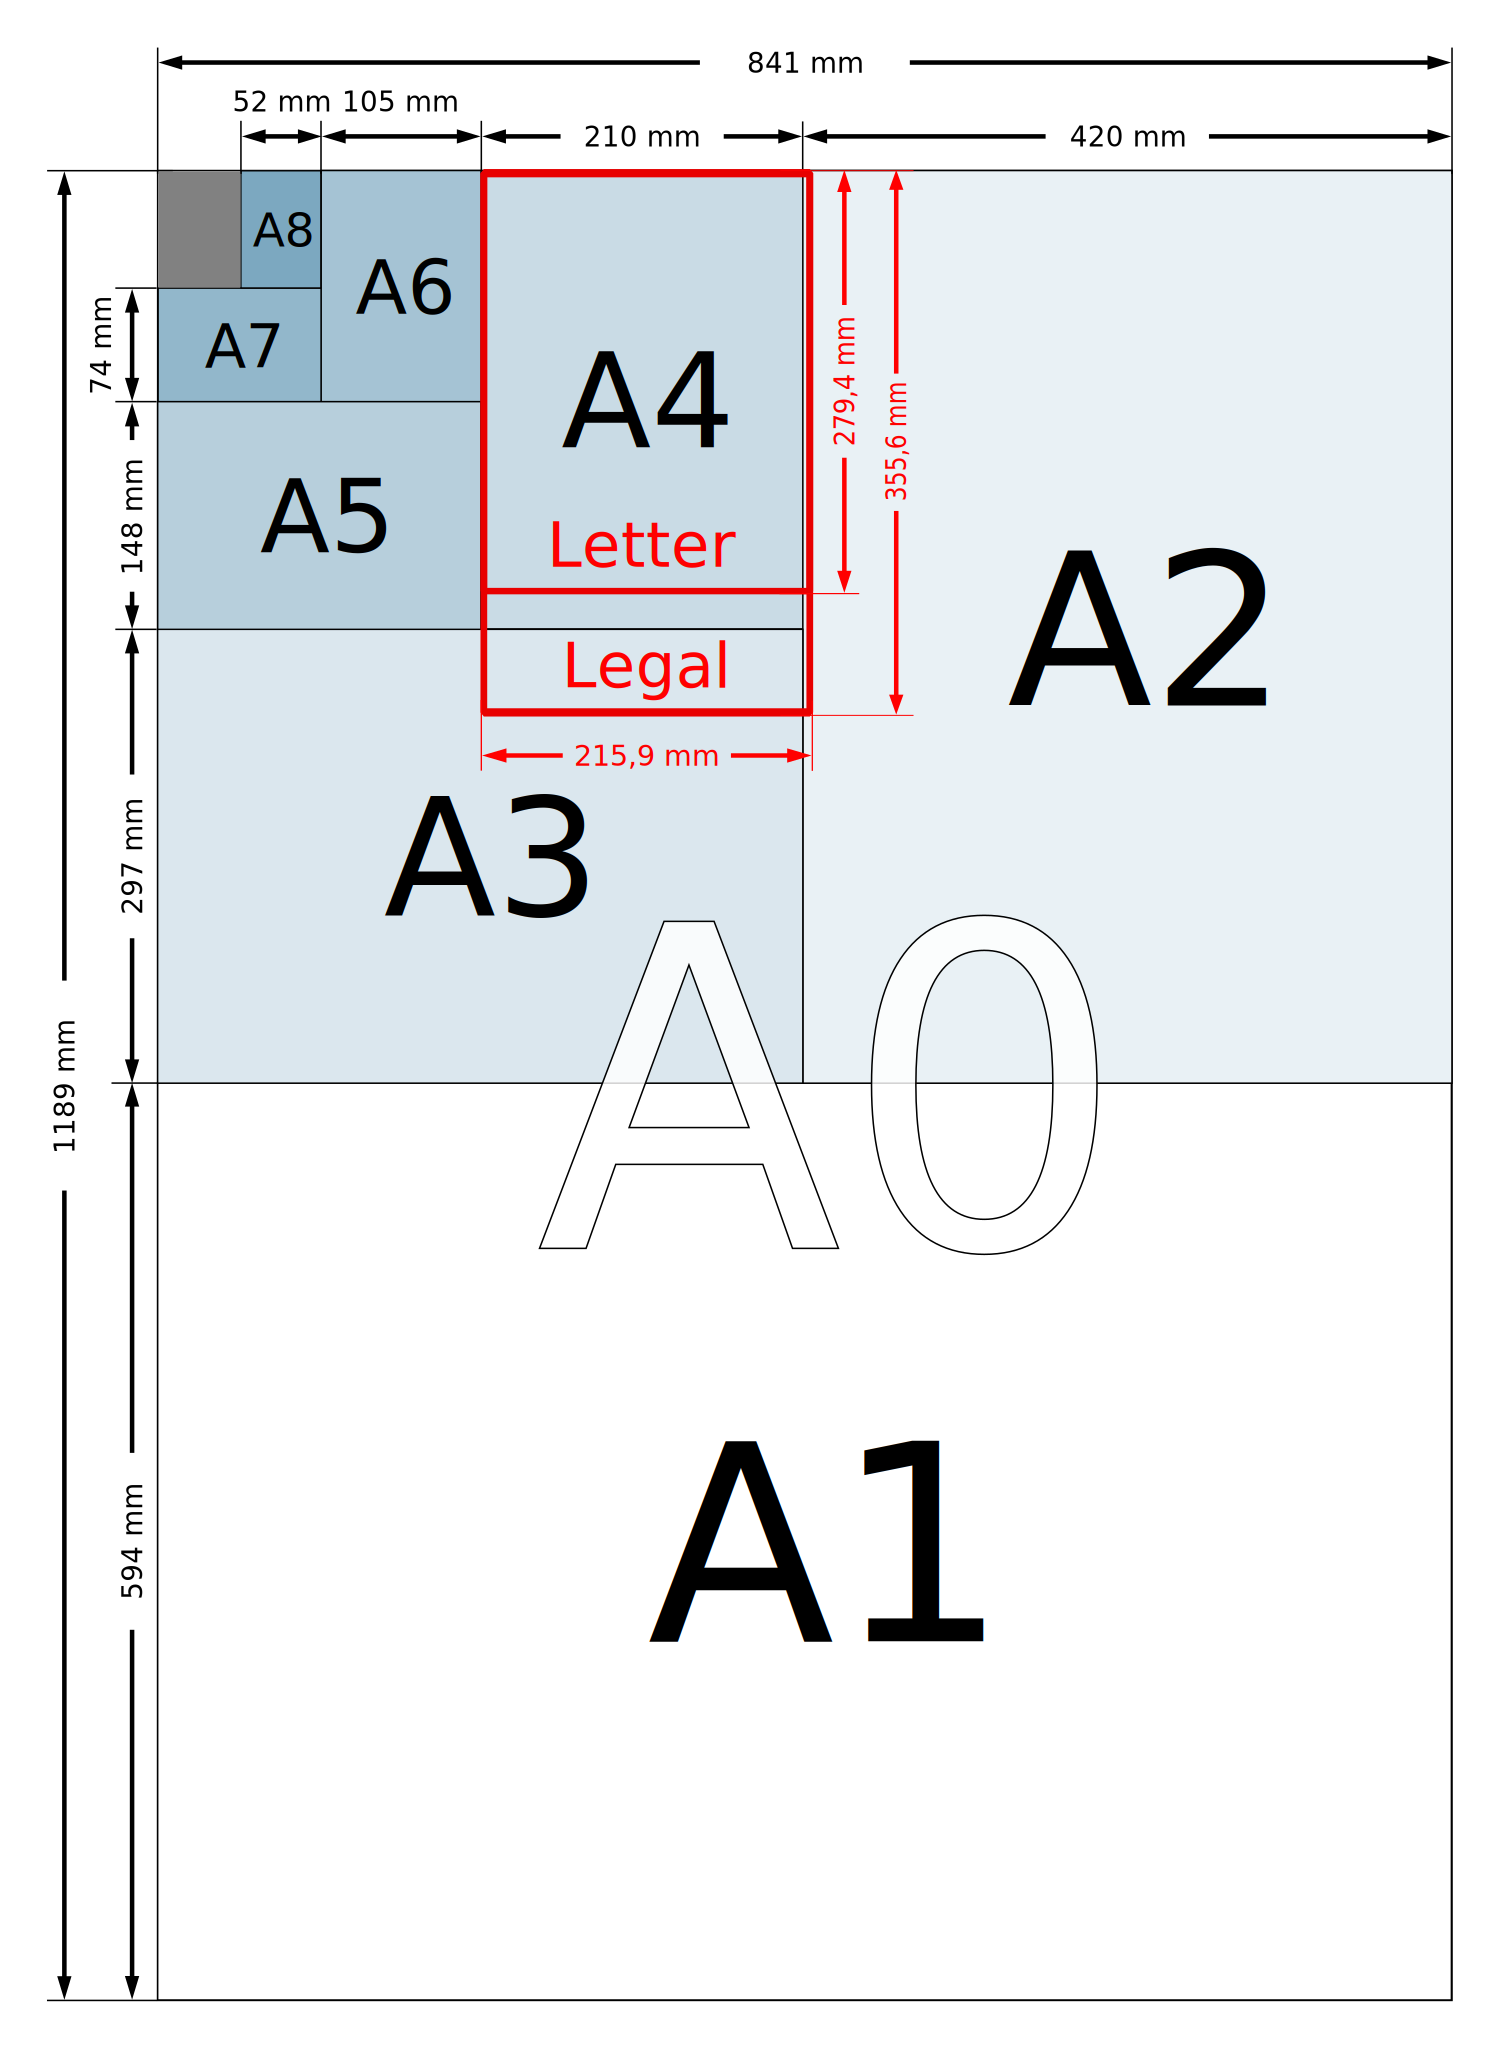
\includegraphics[width=\textwidth,height=.7\textheight,keepaspectratio]{A_size_illustration2_with_letter_and_legal}

      Tamaños ISO 216 A (en.wikipedia.org, <<ISO 216>>)
    \end{center}

    \column{.5\textwidth}
    \begin{itemize}
    \item A0 (841mm $\times$ 1189mm) es popular en Europa: ocupa 4 A4
      de alto y 4 A4 de ancho
    \item En eventos fuera de Europa, puede que se usen medidas
      imperiales, como 2 $\times$ 4 pies, por ejemplo
    \end{itemize}
  \end{columns}
\end{frame}

\begin{frame}{Materiales habituales}
  \hypersetup{colorlinks,linkcolor=blue}

  \begin{block}{Papel: barato, mejor impresión}
    \begin{itemize}
    \item Antes era común pegar fotos y texto sobre una cartulina,
      pero hoy en día lo normal es mandar a imprimir un cartel
    \item Si pensabais imprimir 16 A4 y juntarlos con cinta
      adhesiva... \href{http://www.flickr.com/photos/damienclauzel/4465767871/}{pensadlo
        bien} (bueno, eso era un borrador)
    \item Tened en cuenta el gramaje del papel: un papel de mayor
      calidad aguantará mejor el transporte y puede ser reutilizable
    \item Laminar el papel es buena idea, pero lo hará menos flexible
      y más difícil de transportar (¡cuidado al coger el vuelo!)
    \end{itemize}
  \end{block}

  \begin{block}{Lona o vinilo: algo más cara, pero mucho más resistente}
    \begin{itemize}
    \item Es mucho más resistente y flexible, y no excesivamente cara
    \item Cuidado con pósters con gráficos vectoriales: las líneas
      tienden a correrse si no se seca bien en la imprenta
    \end{itemize}
  \end{block}

\end{frame}

\begin{frame}{Montaje de un póster}

  \begin{block}{Sobre superficie: cinta adhesiva normal}
    Resulta poco estética, al verse desde fuera. Si el póster es de
    papel, puede retirar parte de la tinta al quitarse.
  \end{block}

  \begin{block}{Sobre superficie: cinta adhesiva de doble cara}
    No se ve desde fuera y no retirará nada visible al quitarse. De
    todos modos, si es de papel, cuidado al quitarlo: se podría
    rasgar.
  \end{block}

  \begin{block}{Montado a nivel de suelo: lona y ojales}
    Si tiene que ir montado a nivel de suelo, normalmente se
    enganchará a un armazón, por lo que necesitaréis un cartel de lona
    o vinilo con los
    \href{http://www.printcolorweb.com/spa/item/index.html?msgOrigen=9\&msgValor=58\&CODART=lona}{ojales
      apropiados}
  \end{block}
  
\end{frame}

\section{Defensa}

\begin{frame}{¿Qué hacer y no hacer el día de la sesión?}
  % aseo, aspecto físico, ropa, lenguaje corporal

  % forma de hablar - y cantidad de tiempo que se habla
\end{frame}

\begin{frame}{Materiales de apoyo}
  % tarjetas de visita

  % folletos (dípticos, trípticos)

  % muestras relacionadas con la investigación
\end{frame}

\section[Ejemplos]{Ejemplos de pósters buenos... y no tanto}
\label{sec:posters}

\begin{frame}{Pósters malos}
  
\end{frame}

\begin{frame}{Pósters buenos}
  
\end{frame}

\appendix

\begin{frame}{Para aprender más}
  \framesubtitle{Cuidado: no todos los ejemplos son buenos}

  \begin{thebibliography}{10}
    \beamertemplatearticlebibitems
    \bibitem{y} Purrington, C.B.
      \newblock Designing conference posters.
      \newblock {\small\url{http://colinpurrington.com/tips/academic/posterdesign}}

    \bibitem{x} Colorado State University.
      \newblock Writing Guide: Poster Sessions.
      \newblock {\small\url{http://writing.colostate.edu/guides/speaking/poster/}}

    \bibitem{z} Flickr.com.
      \newblock Grupo <<Poster sessions>>.
      \newblock {\small\url{http://www.flickr.com/groups/postersessions/}}

    \bibitem{w} Faculty of 1000.
      \newblock F1000Posters Open Access archive.
      \newblock {\small\url{http://f1000.com/posters}}
  \end{thebibliography}
\end{frame}

\begin{frame}{Fin de la presentación}
  \begin{center}
    {\Huge ¡Gracias por su atención!}

    \vspace{3em}

    {\Large
      \href{mailto:antonio.garciadominguez@uca.es}{antonio.garciadominguez@uca.es}}
  \end{center}
\end{frame}

\end{document}
